\documentclass[12pt]{article}

\usepackage{amsmath,amsthm,amsfonts,amssymb,amsxtra}
\usepackage{tikz,array}
\usetikzlibrary{arrows}
\renewcommand{\theenumi}{(\alph{enumi})} 
\renewcommand{\labelenumi}{\theenumi}

\pagestyle{empty}
\setlength{\textwidth}{7in}
\setlength{\oddsidemargin}{-0.5in}
\setlength{\topmargin}{-1.0in}
\setlength{\textheight}{9.5in}

\theoremstyle{definition}
\newtheorem{problem}{Problem}

\begin{document}

\noindent{\large\bf MATH 242}\hfill{\large\bf Test \#5}\hfill{\large\bf Fall 2018}\hfill{\large\bf Page 1/6}\hrule

\bigskip
\begin{center}
  \begin{tabular}{|ll|}
    \hline & \\
    {\bf Name: } & \makebox[12cm]{\hrulefill}\\
           & \\
    {\bf VIP ID:} & \makebox[12cm]{\hrulefill}\\ & \\
                                                                                                            \hline
  \end{tabular}
\end{center}
\begin{itemize}
\item Write your name and your VIP ID in the space provided above.
\item The test has six (6) pages, including this one.
\item Show sufficient work to justify all answers unless otherwise stated in the problem.  Correct answers with
  inconsistent work may not be given credit.
\item Credit for each problem is given at the right of each problem number.
\end{itemize}
\hrule

\begin{center}
  \begin{tabular}{|c|c|c|}
    \hline
    &&\\
       {\large\bf Page} & {\large\bf Max} & {\large\bf Points} \\
    &&\\
       \hline
    &&\\
       {\Large 2} & \Large 30 & \\
    &&\\
       \hline
    &&\\
       {\Large 3} & \Large 30 & \\
    &&\\
       \hline
    &&\\
       {\Large 4} & \Large 20 & \\
    &&\\
       \hline
    &&\\
       {\Large 5} & \Large 20 & \\
    &&\\
       \hline\hline
    &&\\
       {\large\bf Total} & \Large 100 & \\
    &&\\
       \hline
  \end{tabular}
\end{center}
\newpage

%%%%%%%%%%%%%%%%%%%%%%%%%%%%%%%%%%%%% Page 2
\noindent{\large\bf MATH 242}\hfill{\large\bf Test \#5}\hfill{\large\bf Fall 2018}\hfill{\large\bf Page 2/6}\hrule

\bigskip
\begin{problem}[30 pts---10 pts each part]
  A body with mass 0.5~kg is attached to the end of a spring that is stretched 2~m by a force of 100~N.  It is set in
  motion one meter to the right, and moving to the left at that time with an initial velocity of 5~m/s.
  \begin{enumerate}
  \item Find the position function of the body.
    \vspace{3cm}
    \begin{flushright}
      \begin{tikzpicture}
        \draw (-0.75cm, 0.5cm) node{$x(t)=$};
        \draw (0cm,-0.2cm) rectangle (5cm,1.2cm);
      \end{tikzpicture}
    \end{flushright}
  \item Indicate the amplitude, frequency, period of oscillation and time lag of this motion.
    \vspace{3cm}
    \begin{flushright}
      \begin{tikzpicture}
        \draw (-1.2cm, 0.5cm) node{Amplitude:};
        \draw (0cm,-0.2cm) rectangle (2cm,1.2cm);
        \begin{scope}[xshift=4.5cm]
          \draw (-1.2cm, 0.5cm) node{Frequency:};
          \draw (0cm,-0.2cm) rectangle (2cm,1.2cm);
        \end{scope}
        \begin{scope}[xshift=8.5cm]
          \draw (-1cm, 0.5cm) node{Period:};
          \draw (0cm,-0.2cm) rectangle (2cm,1.2cm);
        \end{scope}
        \begin{scope}[xshift=13cm]
          \draw (-1cm, 0.5cm) node{Time lag:};
          \draw (0cm,-0.2cm) rectangle (2cm,1.2cm);
        \end{scope}
      \end{tikzpicture}
    \end{flushright}
  \item Sketch the solution curve.  Make sure to label all relevant information (amplitude, time lag and period).
  \end{enumerate}
\end{problem} 

\newpage

%%%%%%%%%%%%%%%%%%%%%%%%%%%%%%%%%%%%% Page 3
\noindent{\large\bf MATH 242}\hfill{\large\bf Test \#5}\hfill{\large\bf Fall 2018}\hfill{\large\bf Page 3/6}\hrule

\bigskip
\begin{problem}[30 pts---10 pts each part]
  The mass and spring of the previous problem are now attached also to a dashpot that provides 1~N of resistance for
  each meter per second of velocity.  The mass is set in motion with the same initial position and initial velocity as
  before.
  \begin{enumerate}
  \item Find the position function of the body.
    \vspace{3cm}
    \begin{flushright}
      \begin{tikzpicture}
        \draw (-0.75cm, 0.5cm) node{$x(t)=$};
        \draw (0cm,-0.2cm) rectangle (5cm,1.2cm);
      \end{tikzpicture}
    \end{flushright}
  \item Indicate the amplitude, the new frequency, pseudoperiod of motion and new time lag of this motion.
    \vspace{3cm}
    \begin{flushright}
      \begin{tikzpicture}
        \draw (-1.2cm, 0.5cm) node{Amplitude:};
        \draw (0cm,-0.2cm) rectangle (2cm,1.2cm);
        \begin{scope}[xshift=4.4cm]
          \draw (-1.2cm, 0.5cm) node{Frequency:};
          \draw (0cm,-0.2cm) rectangle (2cm,1.2cm);
        \end{scope}
        \begin{scope}[xshift=9.3cm]
          \draw (-1.4cm, 0.5cm) node{Pseudoperiod:};
          \draw (0cm,-0.2cm) rectangle (2cm,1.2cm);
        \end{scope}
        \begin{scope}[xshift=13.5cm]
          \draw (-1cm, 0.5cm) node{Time lag:};
          \draw (0cm,-0.2cm) rectangle (2cm,1.2cm);
        \end{scope}
      \end{tikzpicture}
    \end{flushright}
  \item Sketch the solution curve.  Make sure to label all relevant information (amplitude, time lag and pseudoperiod).
  \end{enumerate}
\end{problem} 
\newpage

%%%%%%%%%%%%%%%%%%%%%%%%%%%%%%%%%%%%% Page 4
\noindent{\large\bf MATH 242}\hfill{\large\bf Test \#5}\hfill{\large\bf Fall 2018}\hfill{\large\bf Page 4/6}\hrule

\bigskip
\begin{problem}[20 pts---10 pts each part]
  Consider an undamped forced motion with equation $x''+9x=80\cos 5t,$ which is set in motion with $x(0)=x'(0)=0$.
  \begin{enumerate}
  \item Find the position function of the body.
    \vspace{4cm}
    \begin{flushright}
      \begin{tikzpicture}
        \draw (-0.75cm, 0.5cm) node{$x(t)=$};
        \draw (0cm,-0.2cm) rectangle (5cm,1.2cm);
      \end{tikzpicture}
    \end{flushright}
  \item Sketch the solution curve.  Indicate clearly how far the mass moves to the right before starting back toward the
    origin (show all necessary work to find this value)
  \end{enumerate}  
\end{problem}
\newpage

%%%%%%%%%%%%%%%%%%%%%%%%%%%%%%%%%%%%% Page 5
\noindent{\large\bf MATH 242}\hfill{\large\bf Test \#5}\hfill{\large\bf Fall 2018}\hfill{\large\bf Page 5/6}\hrule

\bigskip
\begin{problem}[10 pts]
  A motorboat starts from rest.  Its motor provides a constant acceleration of $4~\mathrm{ft}/\mathrm{s}^2$, but water
  resistance causes a deceleration of $0.0025v^2$.  What is the \emph{limiting velocity} of the boat?
  \vspace{5cm}
  \begin{flushright}
    \begin{tikzpicture}
      \draw (-0.75cm, 0.5cm) node{$v=$};
      \draw (0cm,-0.2cm) rectangle (5cm,1.2cm);
    \end{tikzpicture}
  \end{flushright}
\end{problem}

\hrule
\begin{problem}[10 pts]
  An arrow is shot straight upward from the ground with an initial velocity of $160~\mathrm{ft}/\mathrm{s}$.  It
  experiences both the deceleration of gravity and deceleration $0.00125v^2$ due to air resistance.  How high in the air
  does it go?
  \vspace{10cm}
  \begin{flushright}
    \begin{tikzpicture}
      \draw (-0.75cm, 0.5cm) node{$h=$};
      \draw (0cm,-0.2cm) rectangle (5cm,1.2cm);
    \end{tikzpicture}
  \end{flushright}
\end{problem}
\newpage

%%%%%%%%%%%%%%%%%%%%%%%%%%%%%%%%%%%%% Page 6
\noindent{\large\bf MATH 242}\hfill{\large\bf Test \#5}\hfill{\large\bf Fall 2018}\hfill{\large\bf Page 6/6}\hrule

\bigskip
\begin{center}
  \begin{tikzpicture}
    \node[scale=0.97]{
      \begin{tabular}{|m{1.2cm}|m{4.3cm}l||m{2.1cm}|m{4.3cm}l|}
        \hline
        $f(x)$\raisebox{0.5cm} & $\mathcal{L}\{f\}=\int_0^\infty e^{-sx}f(x)\, dx$\raisebox{0.5cm} & &
                                                                                                       \raisebox{0.5cm} & \raisebox{0.5cm} & \\[0.4cm] 
        \hline \hline
        $1$ & $\dfrac{1}{s}$\raisebox{0.6cm} & $s>0$ &
                                                       $cf(x)\pm g(x)$ & $cF(s) \pm G(s)$\raisebox{0.4cm} & $s>max(a,b)$ \\[0.4cm]
        \hline
        $x^n$ & $\dfrac{n!}{s^{n+1}}$\raisebox{0.6cm} & $s>0$ & $e^{\alpha x}f(x)$ & $F(s-\alpha)$\raisebox{0.4cm} & $s>a+\alpha$ \\[0.4cm]
        \hline
        $e^{\alpha x}$ & $\dfrac{1}{s-\alpha}$\raisebox{0.6cm} & $s>\alpha$ &
                                                                              $x^n f(x)$ & $(-1)^n F^{(n)}(s)$\raisebox{0.4cm} & $s>a$ \\[0.4cm]
        \hline
        $\sin \beta x$ & $\dfrac{\beta}{s^2+\beta^2}$\raisebox{0.6cm} & $s>0$ & $f'(x)$ & $s F(s) -f(0)$\raisebox{0.4cm} & \\[0.4cm]
        \hline
        $\cos \beta x$ & $\dfrac{s}{s^2+\beta^2}$\raisebox{0.6cm} & $s>0$ &$f''(x)$\raisebox{0.4cm} & $s^2F(s) - sf(0)  - f'(0)$ & \\[0.4cm]
        \hline
      \end{tabular} };
  \end{tikzpicture}
\end{center}

\end{document}

%%% Local Variables:
%%% mode: latex
%%% TeX-master: t
%%% End:
